\documentclass{ohm_project_description}

\projecttitle{AI-based Processing of Traffic Monitoring Footage}
\projectauthor{Labor für mobile Robotik}
\projectdate{2025}

\begin{document}

\maketitle
\thispagestyle{fancy}

\vspace*{-2.5cm}
\begin{figure}[h!]
    \centering
    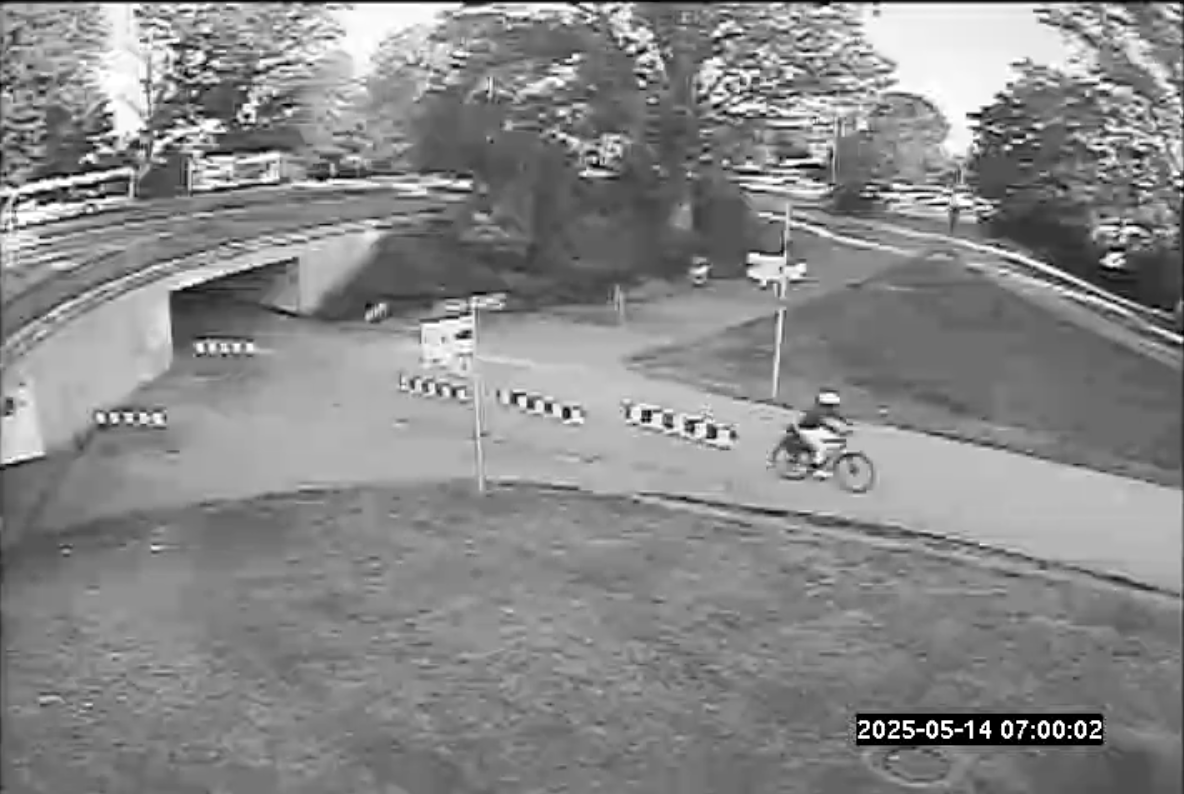
\includegraphics[height=4cm]{img/traffic_cam.png}
\end{figure} 


The goal of the project is the development of algorithms for the automatic processing and analysis of traffic monitoring footage. The focus is on detecting and tracking traffic participants in pre-recorded, low-resolution video footage. Objects in the videos need to be identified and tracked over time. Additionally, an algorithm for the detection of near-collisions should be developed. \\

This project will be conducted in collaboration with the Laboratory for Transportation (Prof. Dr. Matthias Bohlinger). 

\section*{Work Packages}
\begin{itemize}[leftmargin=0.5cm]
    \setlength\itemsep{.1em}
    \item Research and selection of suitable algorithms for object detection and tracking in low-resolution video footage
    \item Implementation of the selected algorithms
    \item Implementation of an algorithm for near-collision detection
    \item Evaluation of the implemented algorithms on traffic monitoring footage
    \item (optional) Implementation of a web-based analysis tool for visualizing the results of the algorithms
\end{itemize}

\section*{Requirements}
\begin{itemize}[leftmargin=0.5cm]
    \setlength\itemsep{.1em}
    \item Knowledge of a higher-level programming language (e.g., Python, C++)
    \item Knowledge of machine learning and deep learning (demonstrated ideally through completing a suitable Deep Learning course from the university curriculum)
\end{itemize}

\vspace{0.5cm}
This topic is ideally suited as a a Bachelor's or Master's thesis. However, an extended version can also be worked on as a project work for two to three students.


\vfill
\textcolor{ohm_red}{\rule{\linewidth}{0.4mm}}
\textbf{\textcolor{ohm_red}{Labor für mobile Robotik}} \\
\begin{tabular}{@{}ll}
\textbf{Supervisor:} & Prof. Dr. Enrico Schröder \\
\textbf{E-Mail:}   & \href{mailto:enrico.schroeder@th-nuernberg.de}{enrico.schroeder@th-nuernberg.de} \\
\end{tabular}

\end{document}